\documentclass{article}
\usepackage[a4paper, margin=1.5cm]{geometry}
\usepackage[slovene]{babel}
\usepackage[utf8]{inputenc}
\renewcommand*\familydefault{\ttdefault}
\renewcommand*\familydefault{\sfdefault}
\usepackage{graphicx}
\usepackage{xcolor}
\usepackage{nopageno}
\usepackage{listings}
\usepackage{setspace}
\usepackage{enumitem}
\usepackage{wrapfig}
\usepackage{color,soul}
\usepackage{enumitem}
\setlist[itemize]{noitemsep}
\usepackage{multicol}
\setlength{\columnsep}{0cm}

\usepackage[usefilenames,RMstyle={Medium,Semibold},SSstyle={Medium,Semibold},TTstyle={Medium,Semibold},DefaultFeatures={Ligatures=Common}]{plex-otf}
\lstdefinestyle{mystyle}{ 
    basicstyle=\ttfamily\footnotesize
}
\lstset{style=mystyle}

\newlength\tindent
\setlength{\tindent}{\parindent}
\setlength{\parindent}{0pt}
\renewcommand{\indent}{\hspace*{\tindent}}

\definecolor{0orange}{RGB}{255,153,51}
\definecolor{1yellow}{RGB}{255,255,0}
\definecolor{2pink}{RGB}{255,102,255}
\definecolor{3green}{RGB}{102,255,102}
\definecolor{4blue}{RGB}{102,178,255}


\RequirePackage[framemethod=default]{mdframed}
\definecolor{infoshadecolor}{RGB}{174,214,241}
\definecolor{infocolor}{RGB}{52,152,219}
\definecolor{warningshadecolor}{RGB}{245,183,177}
\definecolor{warningcolor}{RGB}{231,76,60}
\definecolor{titleshadecolor}{RGB}{255,255,255}
\definecolor{titlecolor}{RGB}{255,255,255}
\definecolor{codeshadecolor}{RGB}{236, 239, 241}
\definecolor{codecolor}{RGB}{176,190,197}
\definecolor{textmyshadecolor}{RGB}{255,255,255}
\definecolor{textmycolor}{RGB}{0,0,0}

\newmdenv[
    skipabove=0pt,
    skipbelow=0pt,
    rightline=false,
    leftline=true,
    topline=false,
    bottomline=false,
    % linecolor=infocolor,
    backgroundcolor=infoshadecolor,
    innerleftmargin=5pt,
    innerrightmargin=5pt,
    innertopmargin=5pt,
    leftmargin=0cm,
    rightmargin=0cm,
    linewidth=4pt,
    innerbottommargin=5pt
]{infoBox}
\newmdenv[
    skipabove=0pt,
    skipbelow=0pt,
    rightline=false,
    leftline=true,
    topline=false,
    bottomline=false,
    % linecolor=warningcolor,
    backgroundcolor=warningshadecolor,
    innerleftmargin=5pt,
    innerrightmargin=5pt,
    innertopmargin=5pt,
    leftmargin=0cm,
    rightmargin=0cm,
    linewidth=4pt,
    innerbottommargin=5pt
]{warningBox}
\newmdenv[
    skipabove=0pt,
    skipbelow=0pt,
    rightline=false,
    leftline=true,
    topline=false,
    bottomline=false,
    % linecolor=codecolor,
    backgroundcolor=codeshadecolor,
    innerleftmargin=5pt,
    innerrightmargin=5pt,
    innertopmargin=0pt,
    leftmargin=0cm,
    rightmargin=0cm,
    linewidth=4pt,
    innerbottommargin=0pt
]{codeBox}
\newmdenv[
    skipabove=0pt,
    skipbelow=0pt,
    rightline=false,
    leftline=true,
    topline=false,
    bottomline=false,
    % linecolor=2pink,
    backgroundcolor=textmyshadecolor,
    innerleftmargin=5pt,
    innerrightmargin=0pt,
    innertopmargin=2pt,
    leftmargin=0cm,
    rightmargin=10pt,
    linewidth=4pt,
    innerbottommargin=2pt
]{textBox}

\newenvironment{infobox}[1][]{\begin{infoBox}[linecolor=#1]}{\end{infoBox}}
\newenvironment{warnbox}[1][]{\begin{warningBox}[linecolor=#1]}{\end{warningBox}}
% \newenvironment{titlebox}{\begin{titleBox}\begin{Large}\begin{bfseries}}{\end{bfseries}\end{Large}\end{titleBox}}
\newenvironment{codebox}[1][]{\begin{codeBox}[linecolor=#1]}{\end{codeBox}}
\newenvironment{textbox}[1][]{\begin{textBox}[linecolor=#1]}{\end{textBox}}

\newcommand{\titlebox}[1]{
    \vspace{3pt}
    \begin{large}
    \bfseries
    #1
    \end{large}
}

\newcommand{\standout}[1]{
    \ul{#1}
}

\setul{0.2ex}{0.3ex}
\setulcolor{red}




\begin{document}
\begin{multicols*}{2}

%\begin{center}
    
\includegraphics[width=0.6\linewidth]{images/Git-Logo-2Color.png} 
%\end{center}

\titlebox{\colorbox{black}{\textcolor{white}{Osnovno}}}

\begin{textbox}[black]
Praviloma ima git repozitorij ali \standout{repo} tri nivoje beleženja sprememb:

\begin{itemize}[leftmargin=10pt]
    \item \standout{struktura datotek} datoteke v mapah, ki so shranjene na disku
    \item \standout{staging} vmesna stopnja kamor dodamo datoteke, ki jih želimo dodati v enem commit-u
    \item \standout{repo} končna stopnja, kjer so beležene vse spremembe od nastanka repota
\end{itemize}
Nivoji beleženja sprememb in nekateri ukazi za prehajanje med njimi:
\begin{center}
    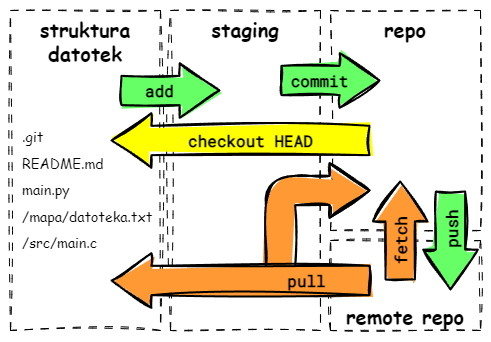
\includegraphics[width=0.8\linewidth]{images/git-skica.png}
\end{center}
\end{textbox}

\titlebox{\colorbox{black}{\textcolor{white}{Prenašanje repozitorija}}}

\begin{textbox}[black]
Kadar želimo s strežnika prenesti nov repo:
\end{textbox}

\begin{codebox}[black]
\begin{lstlisting}
git clone <url/repozitorija>
git clone https://github.com/jankoslavic/pypinm.git
\end{lstlisting}
\end{codebox}

\titlebox{\colorbox{black}{\textcolor{white}{SSH}}}

\begin{textbox}[black]
Protokol SSH omogoča varen dostop do oddaljenih repozitorijev bre uporabniškega imena in gesla.\\
SSH ne potrebujemo, kadar želimo prenesti javni repo.
\end{textbox}

\begin{infobox}[black]
SSH ključ je sestavljen iz dveh delov:
\begin{itemize}[leftmargin=10pt]
    \item \textbf{privatni} [\lstinline{id_ed25519}] predstavlja tvojo podpis
    \item \textbf{javni} [\lstinline{id_ed25519.pub}] omogoča preverjanje, ali je bil nek dokument podpisan s tvojim privatnim ključem
\end{itemize}
\end{infobox}

\begin{warnbox}[black]
POZOR! Nikoli ne nalagaj ali pošiljaj svojega privatnega ključa (datoteka brez končnice).
\end{warnbox}

\begin{textbox}[black]
Najprej generiramo nov par ED25519 ključev:
\end{textbox}

\begin{codebox}[black]
\begin{lstlisting}
ssh-keygen -t ed25519 -C "<komentar>"
\end{lstlisting}
\end{codebox}

\begin{textbox}[black]
Na nadaljnja vprašanja lahko odgovorimo z privzetimi vrednostmi.\\
Javni SSH ključ kopiramo z naslednjim ukazom:
\end{textbox}

\begin{codebox}[black]
\begin{lstlisting}
cat ~/.ssh/id_ed25519.pub | clip         # Windows
xclip -sel clip < ~/.ssh/id_ed25519.pub  # Linux
\end{lstlisting}
\end{codebox}

\begin{textbox}[black]
SSH ključ nato vnesemo na spletni strani GitHub.com.
[\lstinline{Settings -> SSH keys -> Add new key}]
\end{textbox}

\vfill\null
\columnbreak
\titlebox{\colorbox{black}{\textcolor{white}{Globalne nastavitve}}}

\begin{textbox}[black]
    Nastavi e-mail in Uporabniško ime uporabnika:
\end{textbox}

\begin{codebox}[black]
\begin{lstlisting}
git config --global user.name "<uporabnisko_ime>"
git config --global user.email "<tvoj@email.com>"
\end{lstlisting}
\end{codebox}

\titlebox{\colorbox{black}{\textcolor{white}{Ustvarjanje novega repoziritorija}}}

\begin{codebox}[black]
\begin{lstlisting}
git init
\end{lstlisting}
\end{codebox}

\begin{codebox}[black]
\begin{lstlisting}
git remote add <remote_name> <remote_repo_url>
git remote add origin git@github.com:User/repo.git
\end{lstlisting}
\end{codebox}

%\vfill\null
%\columnbreak
\titlebox{\colorbox{black}{\textcolor{white}{Workflow}}}

\begin{textbox}[black]
\begin{center}
    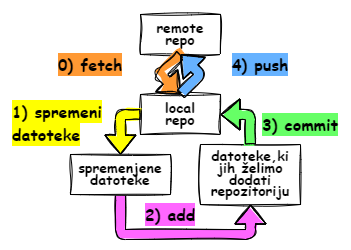
\includegraphics[width=0.8\linewidth]{images/git-workflow.png}
\end{center}
\end{textbox}

\titlebox{\titlebox{\colorbox{2pink}{\textcolor{black}{Dodajanje sprememb}}}}
\begin{textbox}[2pink]
Ko smo opravili \colorbox{1yellow}{spremembe datotek} jih pričnemo pripravljati v \standout{staging} area.

Dodamo lahko: datoteke poimensko, celotno mapo vse spremembe:
\end{textbox}

\begin{codebox}[2pink]
\begin{lstlisting}
git add <ime/datoteke>
git add src/main.py        # Ena datoteka
git add src                # Celotna mapa
git add *                  # Vse spremembe
\end{lstlisting}
\end{codebox}

\begin{textbox}[2pink]
Predhodno izbrisane datoteke lahko dodamo z ukazom \lstinline{add}. Z ukazom \lstinline{rm} datoteke hkrati izbrišemo in dodamo spremembe v staging:
\end{textbox}

\begin{codebox}[2pink]
\begin{lstlisting}
git rm <ime_datoteke>
git rm src/main.py
git rm -r <ime/mape>
git rm -r src
\end{lstlisting}
\end{codebox}

\begin{warnbox}[2pink]
POZOR! Ukaz \lstinline{git rm} bo datoteko izbrisal tudi z diska.
\end{warnbox}

\titlebox{\titlebox{\colorbox{3green}{\textcolor{black}{Shranjevanje sprememb}}}}

\begin{textbox}[3green]
Ko smo v staging dodali vse spremembe, ki spadajo v neko zaključeno enoto spremembe zabeležimo v lokalni repozitorij:
\end{textbox}

\begin{codebox}[3green]
\begin{lstlisting}
git commit -m "<komentar>"
git commit -m "Dodana funkcionalnost XZY"
\end{lstlisting}
\end{codebox}

\titlebox{\titlebox{\colorbox{4blue}{\textcolor{black}{Pošiljanje sprememb na strežnik}}}}

\begin{textbox}[4blue]
Spremembe zabeležene v lokalnem repozitoriju posodobimo tudi na srežniku:
\end{textbox}

\begin{codebox}[4blue]
\begin{lstlisting}
git push origin <ime-veje>
git push origin main
\end{lstlisting}
\end{codebox}

\vfill\null
\columnbreak

\begin{minipage}{\columnwidth}
\titlebox{\colorbox{black}{\textcolor{white}{Veje}}}
\begin{textbox}[black]
Veje omogočajo ločeno okolje za urejanje kode. Primer dobre prakse je, da novih funkcionalnosti ne dodajamo neposredno v glavno vejo (običajno: \lstinline{main}). V ta namen dodamo novo vejo (npr.: \lstinline{nova-funkcionalnost}) in novo funkcionalnost razvijamo v tej veji. Ko je nova funkcionalnost končana in testirana jo lahko združimo nazaj v glavno vejo.

Primer nove veje:
\begin{center}
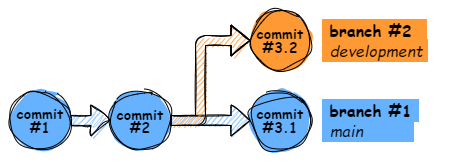
\includegraphics[width=\linewidth]{images/git-branches-checkout.png}
\end{center}
\end{textbox}

\begin{textbox}[black]
Aktivno vejo izberemo z:
\end{textbox}

\begin{codebox}[black]
\begin{lstlisting}
git checkout <ime-veje>
git checkout main
\end{lstlisting}
\end{codebox}

\begin{textbox}[black]
Novo vejo ustvarimo z:
\end{textbox}

\begin{codebox}[black]
\begin{lstlisting}
git branch <ime_veje>
git branch development
\end{lstlisting}
\end{codebox}

\begin{textbox}[black]
Vejo ustvarimo in aktiviramo\\
(ekvivalentno \lstinline{brench} + \lstinline{checkout}):
\end{textbox}

\begin{codebox}[black]
\begin{lstlisting}
git checkout -b <ime-veje>
git checkout -b development
\end{lstlisting}
\end{codebox}

\begin{textbox}[black]
Vejo izbrišemo z:
\end{textbox}

\begin{codebox}[black]
\begin{lstlisting}
git push -d <remote_name> <ime_veje>
git branch -d <ime_veje>
\end{lstlisting}
\end{codebox}
\end{minipage}





%\vfill\null
%\columnbreak

\end{multicols*}
\end{document}
